% $Id$

\section{Target Sources}

Binary neutron star systems, of which a few are known from radio
observations~\cite{Stairs:2004}, are
expected to be distributed spatially in galaxies throughout the universe in
proportion to the blue light luminosity of the various galaxies, with small
corrections to account for the relative metallicities of the galaxies.
While the masses of neutron stars in the few known binary systems are all
near $1.4 M_\odot$, population synthesis simulations suggest that some
systems will have component masses as low as $\sim 1 M_\odot$ and as
high as the theoretical maximum neutron star mass of $\sim 3
M_\odot$~\cite{Belczynski:2002}.  Thus, we search for inspiral signals
from binary systems with component masses in this range.  Note that
higher-mass systems radiate more energy in gravitational waves and can
thus be detected at a greater distance with a given SNR.

When the current LIGO detectors reach their design sensitivities, they
will be capable of detecting inspiral signals from thousands of
galaxies, reaching beyond the Virgo Cluster.  At that time, the
rate of detectable binary neutron star coalescence could be as high
as $0.3$ per year, though it is more likely to be on the order of
$0.1$ per year \cite{Kalogera:2004tn}.
%
For the present analysis, our target population includes the Milky Way
and all significant galaxies within a distance of 3~Mpc,
which is roughly the maximum distance for which a $3 + 3 M_\odot$
inspiral could be detected in coincidence by the L1 and H1
interferometers with a minimal SNR of 6 in H1.  This includes the
entire Local Group of galaxies, whose total mass is dominated by the
Andromeda Galaxy (M31), as well as some galaxies from neighboring
groups.  However, we cannot hope to detect {\em all} inspirals within
this volume, because most systems in the population have lower masses
and because the received signal amplitude is reduced, on average,
depending on the orientation and location of the source relative to
the detector.
%
The total number of binary neutron star
systems within this volume, based on the galactic blue light luminosities
with reddening and metallicity corrections,
is 6.3 times the number of binary neutron star
systems in the Milky Way; we say that our population consists of a total of
$N_{\text{MWEG}}=6.3$ \emph{Milky Way equivalent galaxies} (MWEG).
Table~\ref{t:galaxies} gives the parameters we use for the galaxies in
the target population, and Fig~\ref{f:population} shows a histogram 
of the distribution of the MWEG per effective distance, as well as the reach of 
the LIGO detectors. 

\begin{figure}
\caption{\label{f:population} The upper panel shows the histogram of
the number of Milky Way Equivalent Galaxies ($N_G$) as a function of
effective distance. We indicate the average reach of the best detector
in the First Science Run S1, as well as the average reach of the LIGO
detectors in the Second Science Run. The bottom panel is the
cumulative histogram of the upper panel.}
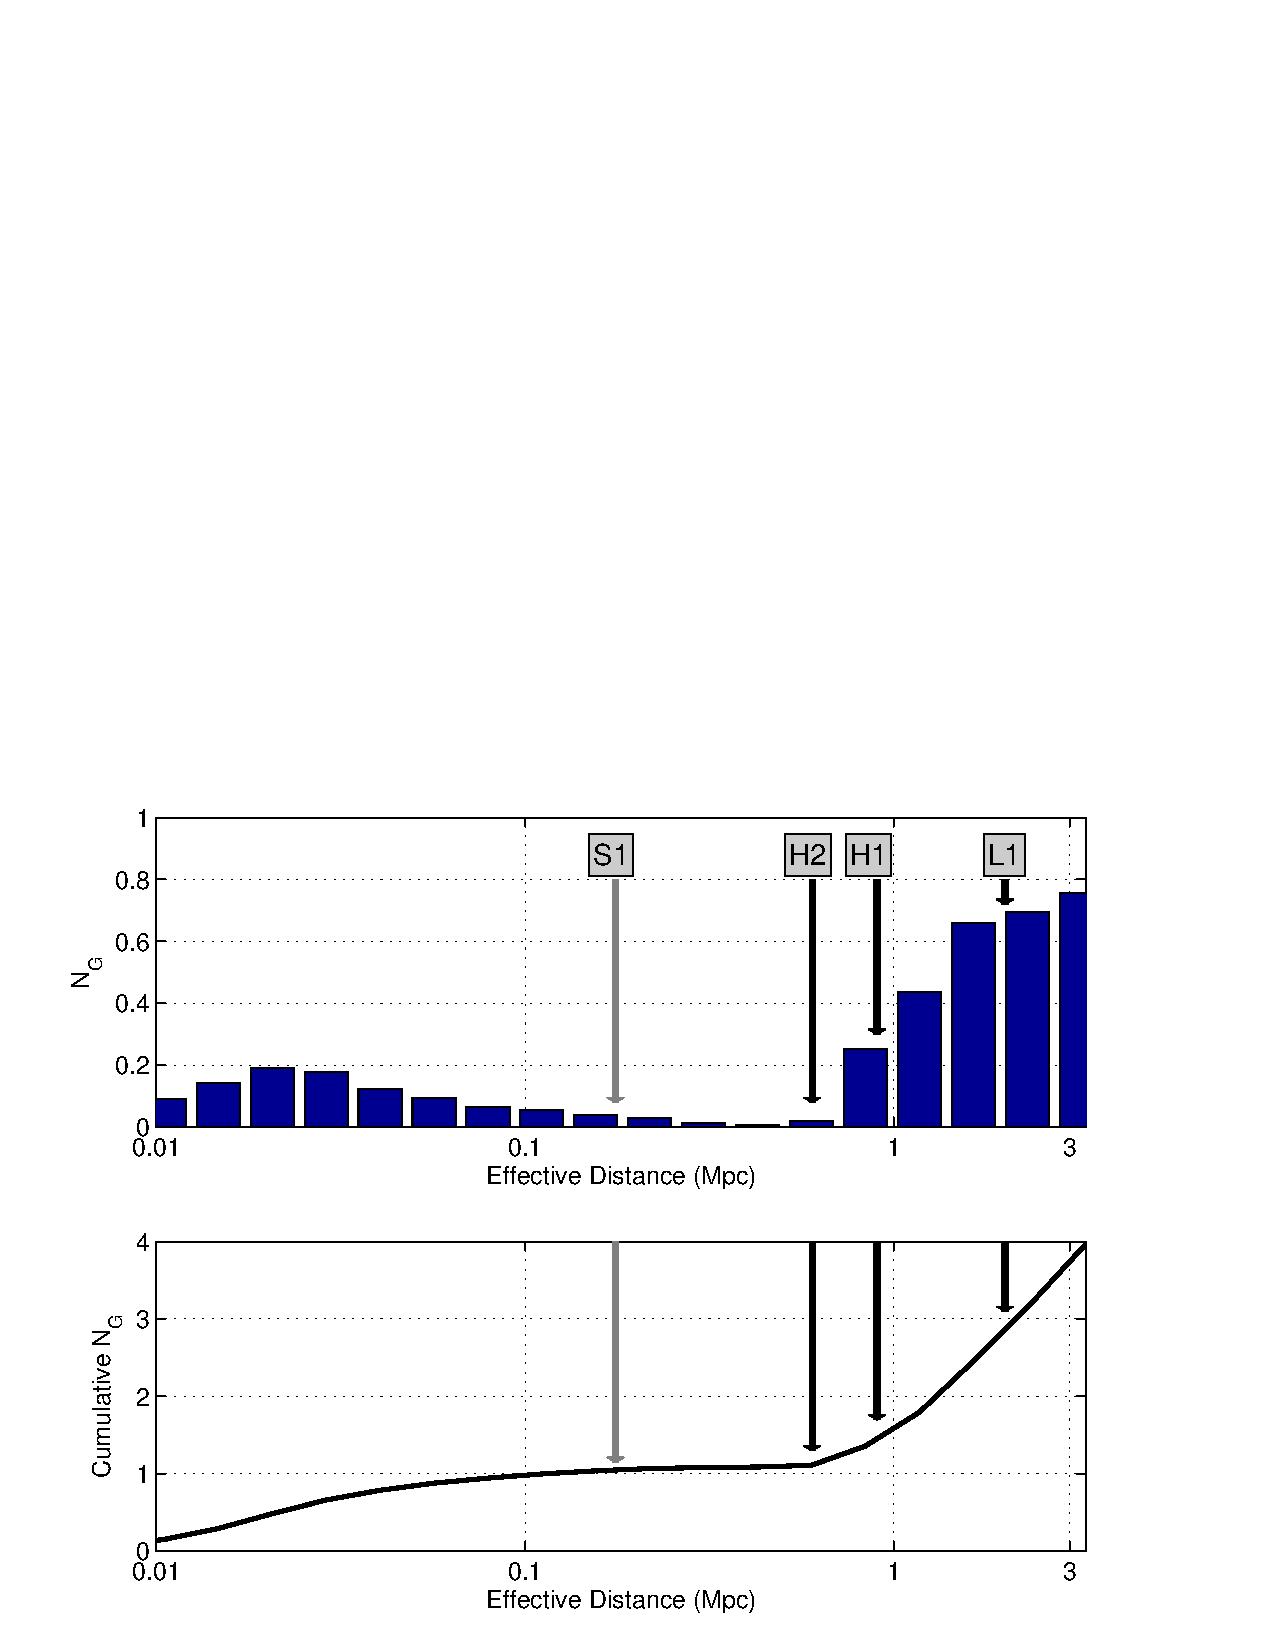
\includegraphics[width=\linewidth]{figures/bns/population}
\end{figure}

\section{Background Estimation}

\section{Triggers and Event Candidates}

\section{Error Analysis}

